\documentclass[11pt, preprint]{article}
\usepackage{hyperref}
\usepackage{rotating}
\usepackage[normalem]{ulem}
\usepackage{environ}
\usepackage{xcolor}
\usepackage{amsmath}

 
\setlength{\footnotesep}{9.6pt}
\setlength{\parskip}{12pt}

\newcounter{thefigs}
\newcommand{\fignum}{\arabic{thefigs}}

\newcounter{thetabs}
\newcommand{\tabnum}{\arabic{thetabs}}

\newcounter{address}

\NewEnviron{answer}[1][]{\color{blue}\expandafter\BODY
{\par \it #1}}

\begin{document}

\begin{center}
  {\bf Radiative Processes in Astrophysics / Problem Set \#3 /
    Answers}
\end{center}


\begin{enumerate}
\item The effect of a polarization filter or a quarter-wave plate, or
  other device affecting the polarization of light is often expressed
  in terms of a 4-by-4 ``Mueller matrix'' ${\bf M}$ defined such that:
  \begin{equation}
    \begin{pmatrix}
      I_{\rm out} \\
      Q_{\rm out} \\
      U_{\rm out} \\
      V_{\rm out} \\
    \end{pmatrix}
    = 
    {\bf M} 
    \cdot
    \begin{pmatrix}
      I_{\rm in} \\
      Q_{\rm in} \\
      U_{\rm in} \\
      V_{\rm in} \\
    \end{pmatrix}
  \end{equation}

  \begin{enumerate}
    \item Imagine a polarization filter that admits only linearly polarized
  light along an axis, taken to be $\theta$ with respect to the
  $x$-axis. What is the Mueller matrix for this filter?

  \begin{answer}
    Since the filter cannot produce or transmit the circular
    polarization, we can write the Mueller matrix as:
    \begin{equation}
      {\bf M} = \begin{pmatrix}
        m_{II} & m_{QI} & m_{UI} & 0 \\
        m_{IQ} & m_{QQ} & m_{UQ} & 0 \\
        m_{IU} & m_{QU} & m_{UU} & 0 \\
        0 & 0 & 0 & 0
      \end{pmatrix}
    \end{equation}

    Recall the relationship between $Q_{\rm out}$, $U_{\rm out}$, and
    the angle $\theta$ needs to be:
    \begin{equation}
      \tan 2\theta  = \frac{U_{\rm out}}{Q_{\rm out}}
    \end{equation}
    If $Q_i=U_i=0$, then the output Stokes vector will be:
    \begin{equation}
      \begin{pmatrix}
        I_o \\
        Q_o \\
        U_o \\
      \end{pmatrix} =
      \begin{pmatrix}
        \frac{1}{2} I_i \\
        \frac{1}{2} I_i \cos 2\theta \\
        \frac{1}{2} I_i \sin 2\theta \\
      \end{pmatrix}
    \end{equation}
    which implies $m_{II}=1/2$, $m_{IQ} = (1/2) \cos 2\theta$, and
    $m_{IU} = (1/2) \sin 2\theta$.

    Now consider $U_i=0$ and $Q_i=I_i$. This means the input electric
    field $E_i$ is linearly polarized in the $x$-direction. The output
    electric field will have the amplitude $|E_i| \cos\theta$, and it
    will have components:
    \begin{eqnarray}
      E_{o, x} &=& E_i \cos\theta\, \cos\theta \cr
      E_{o, y} &=& E_i \cos\theta\, \sin\theta
    \end{eqnarray}
    Then we can use the definition:
    \begin{eqnarray}
      Q_o &=& E_{o,x}^2 - E_{o,y}^2\cr &=& \cos^2\theta \left(\cos^2\theta -
      \sin^2\theta\right) E_i^2\cr &=& \frac{1}{2}\cos 2\theta +
      \frac{1}{2}\cos^2 2\theta
    \end{eqnarray}
    The first term will arise from $m_{IQ}I_i$, so the second term
    demonstrates that $m_{QQ} = (1/2) \cos^2 2\theta$. We also have:
    \begin{equation}
      U_o = 2 E_{o,x}E_{o,y} = 2 E_i^2 \cos^3\theta \sin\theta
      = \frac{1}{2} \sin 2\theta + \frac{1}{2} \cos 2\theta \sin
      2\theta
    \end{equation}
    Again the first term is $m_{IU}I_i$, so the second term is $m_{QU}
    = (1/2) \cos 2\theta \sin 2\theta$. This also follows from the
    relationship between $Q$, $U$, and $\tan 2\theta$.
    We also require
    $I_o^2 = Q_o^2 + U_o^2$ which leads to $m_{QI} = (1/2) \cos
    2\theta$.

    The same set of reasoning applies to the third column of the
    Mueller matrix. If $Q_i=0$ and $U_i = I_i$, then:
    \begin{eqnarray}
      E_{o, x} &=& E_i \cos\theta\, \cos(\theta - \pi/4) \cr
      E_{o, y} &=& E_i \cos\theta\, \sin(\theta - \pi/4)
    \end{eqnarray}
    and: 
    \begin{eqnarray}
      Q_o &=& E_{o,x}^2 - E_{o,y}^2 \cr
      &=& \cos^2\theta
      \left(\cos^2(\theta-\pi/4) -
      \sin^2(\theta-\pi/4) \right) E_i^2 \cr
      &=& \frac{1}{2}\cos 2\theta +
      \frac{1}{2}\cos 2\theta\sin 2\theta
    \end{eqnarray}
    and:
    \begin{equation}
      U_o = 2 E_{o,x} E_{o,y} = \frac{1}{2} \sin 2\theta +
      \frac{1}{2}\sin^2 2\theta
    \end{equation}
    leading to $m_{UQ} = (1/2)\cos 2\theta \sin 2\theta$ and $m_{UU} =
    (1/2) \sin^2 2\theta$.
    We also require
    $I_o^2 = Q_o^2 + U_o^2$ which leads to $m_{UI} = (1/2) \sin
    2\theta$.

    So the Mueller matrix for a linear polarizer in full is:
    \begin{equation}
      {\bf M} = \frac{1}{2} \begin{pmatrix}
        1 & \cos 2\theta & \sin 2\theta & 0 \\
        \cos 2\theta & \cos^2 2\theta & \sin 2\theta\, \cos 2\theta& 0 \\
        \sin 2\theta & \sin 2\theta\, \cos 2\theta& \sin^2 2\theta & 0 \\
        0 & 0 & 0 & 0
      \end{pmatrix}
    \end{equation}
  \end{answer}

  \item Now imagine you use this filter on the observations of some
    object and use a CCD to measure the intensity $I_{\rm
      out}$. Assuming $V=0$ (almost always true in astrophysical
    applications), what is the minimum number of measurements with
    different choices of $\theta$ that you have to do to measure the
    polarization fraction $\Pi$?

    \begin{answer}
      The object has a Stokes vector defined by its $I$, $Q$, and
      $U$. We need to know $\Pi = \sqrt{Q^2 + U^2}/I$. You need to
      make three measurements to determine all three parameters. If
      you measure at $\theta=0$ you will get $I_{\rm out} = I/2 +
      Q/2$, if you measure at $\theta = \pi/4$ you will get $I_{\rm
        out} = I/2 + U/2$, and if you measure at $\theta = \pi/2$ you
      will get $I_{\rm out} = I/2 - Q/2$. You can add the first
      and third measurements to obtain $I$, and subtract them to obtain
      $Q$, and then use the result for $I$ and the second measurement
      to get $U$.
    \end{answer}

  \item Most (all?) polarimetry observations use more than that
    minimum number and much cleverer techniques to observe an object
    through various polarization filters simultaneously. Comment on
    why that is a good idea (beyond any extra total signal-to-noise
    you get from more observations).
    
    \begin{answer}
      It is generally the case that $\Pi$ is less than 1\%. This means
      that the subtraction technique described in (b) depends on $I/2$
      cancelling very well. If you take multiple observations with a
      time gap between them, observing conditions may change and the
      measured $I$ will vary between the observations more than
      1\%. So it is useful to have simultaneous observations of
      multiple polarizations to minimize this effect. Such
      observations can be achieved with a beam-splitter.

      Furthermore, a real filter needs to be calibrated to understand
      its orientation, and since its fixture or rotating element can
      shift or flex over time, and the precise calibration may be a
      function of time or vary slightly from observation to
      observation. The uncertainty in this calibration can be
      mitigated by taking more than the minimum number of angles.
    \end{answer}
  \end{enumerate}

\item Consider an interstellar medium with a constant dust density, so
  that the absorption and scattering factors $\alpha_\nu$ and
  $\sigma_\nu$ are constant. Assume the scattering is isotropic and
  coherent.
  \begin{enumerate}
    \item If from the Earth (i.e. from within this interstellar
      medium) I observe the spectrum of a star at some distance $d$
      (using a narrow aperture including just the light coming from
      exactly the direction of the star). By what factor is the flux I
      measure at frequency $\nu$ affected by the intervening dust?

      \begin{answer}
        The scattering and absorption combined act as an
        overall extinction of 
        $(\alpha_\nu + \sigma_\nu)$, and the resulting equation of
        radiative transfer will be:
        \begin{equation}
          \frac{{\rm d}I_\nu}{{\rm d}s} = -(\alpha_\nu + \sigma_\nu)
          I_\nu + \sigma_\nu J_\nu
        \end{equation}
        Along the ray between us and the star there is no intervening
        emitters (because we used such a narrow aperture; i.e. we
        really are looking at a single ray). Since every part of the
        ray is far away from a star (the sky at each location is
        dark!) the angle-average specific intensity $J_\nu$ is
        extremely small. This means we can neglect the last term
        describing scattering into the line of sight, and solve for:
        \begin{equation}
          I_\nu = I_\nu(0) \exp\left(-(\alpha_\nu + \sigma_\nu)
          s\right).
        \end{equation}
      \end{answer}
    \item Now imagine I observe the total spectrum of a distant galaxy
      from outside, using an aperture that covers all of the light
      coming from the galaxy. Assume the galaxy is spherical and the
      dust and the stars are intermixed randomly, and for simplicity
      they are all the same type of star as in part (a).  If
      $\alpha_\nu = 0$ but $\sigma_\nu$ is significant, how is the
      spectrum affected by the presence of the dust?

      \begin{answer}
        The spectrum will not be affected at all (well, there might be
        Doppler broadening effects). Because there is no absorption
        and the geometry is isotropic, all scattering out of the line of
        sight will be replaced by scattering into the line of sight.
      \end{answer}
    \item If $\sigma_\nu = 0$ but $\alpha_\nu$ is significant, how
      does the effect of dust on the spectrum differ from the effect
      on the single star in part (a)?

      \begin{answer}
        It is largely similar. In this case, all of the absorption is
        internal to the galaxy. Instead of being at a single optical
        depth, the stars will be viewed at a range of optical
        depths, and the total specific intensity will be a sum of all
        those depths.

        The exact form of the resulting absorption is a bit tricky to
        calculate. If the total luminosity at a given wavelength is
        $L_\nu$, then the emission coeffient in some direction
        $\hat{x}$ is:
        \begin{equation}
          j_\nu = \frac{L_\nu}{4\pi V}
        \end{equation}
        where $V$ is the volume of the sphere. We want to calculate
        the effect of absorption on the emergent specific intensity
        from the sphere. This means integrating the $I_\nu$ that
        emerges in direction $\hat{x}$, over the geometrical
        cross-section in the $y$-$z$ plane of the sphere, and
        comparing that result to $L_\nu / 4\pi$. This fractional
        decrement can then be written as:
        \begin{equation}
          f = \frac{3}{4\pi R^3} \int {\rm d}^3\vec{r}
          \exp(-\alpha_\nu s)
        \end{equation}
        where $s$ is the distance from location $\vec{r}$ to the
        surface of the sphere, along the direction $\hat{x}$. We can
        define $b$ as the distance in $y$-$z$ plane from the $x$-axis
        to $\vec{r}$, and define $\phi$ as the polar angle around the
        $x$-axis. Then our coordinate system is defined by $x$, $b$,
        and $\phi$. We then can break up the integral:
        \begin{equation}
          f = \frac{3}{4\pi R^3} \int_0^{2\pi} {\rm d}\phi
          \int_0^R b {\rm d}b \int_{0}^{2x_{\rm m}(b)}
              {\rm d}s \exp(-\alpha s)
        \end{equation}
        where $x_{\rm m} = \sqrt{R^2 - b^2}$. Then
        \begin{eqnarray}
          f &=& \frac{3}{2 R^3}
          \int_0^R b {\rm d}b \int_{0}^{2x_{\rm m}(b)}
              {\rm d}s \exp(-\alpha s) \cr
          &=& \frac{3}{2 R^3}
          \int_0^R b {\rm d}b \left[-\frac{1}{\alpha} 
              \exp(-\alpha s)\right]^{2x_{\rm m}(b)}_0 \cr
          &=& \frac{3}{2 \alpha R^3}
          \int_0^R b {\rm d}b \left(1 - 
              \exp\left(-2 \alpha \sqrt{R^2 - b^2}\right)\right)
        \end{eqnarray}
        With the substitution $x= b /R$:
        \begin{eqnarray}
          f
          &=& \frac{3}{2 \alpha R}
          \int_0^1 x {\rm d}x \left(1 - 
              \exp\left(-2 \alpha R \sqrt{1^2 - x^2}\right)\right)\cr
          &=& \frac{3}{4 \alpha R}
          \left(1 - 2 \int_0^1 x {\rm d}x 
              \exp\left(-2 \alpha R \sqrt{1^2 - x^2}\right)\right)
        \end{eqnarray}
        This is not a simple integral nor is it a common special
        function that I know of. However, we can look at optically
        thin and optically thick limits.

        For $\alpha R\gg 1$, the integral gets vanishingly small so:
        \begin{equation}
          f = \frac{3}{4} \frac{1}{\alpha R}
        \end{equation}
        
        For $\alpha R\ll 1$, we can expand the exponential as a Taylor
        series, and keeping terms to first order (total) in $\alpha R$:
        \begin{eqnarray}
          f
          &=& \frac{3}{4 \alpha R}
          \left(1 - 2 \int_0^1 x {\rm d}x 
              \exp\left(-2 \alpha R \sqrt{1^2 - x^2}\right)\right) \cr
          &=& \frac{3}{4 \alpha R}
          \left[1 - 2 \int_0^1 x {\rm d}x  \left( 1 - 2\alpha R
          \sqrt{1-x^2} + 2 (\alpha R)^2 (1-x^2)\right) \right]\cr
          &=& \frac{3}{4 \alpha R}
          \left( 4 \alpha R \int_0^1 {\rm d}x x \sqrt{1-x^2}
          - 4 (\alpha R)^2 \int_0^1 {\rm d}x x (1-x^2)\right) \cr
          &=& \frac{3}{4 \alpha R}
          \left( \left[- 4 \alpha R \frac{1}{3}\left(1 -
            x^2\right)^{3/2} \right]_0^1
          + \left[4 (\alpha R)^2 \frac{1}{4}\left(1 -
          x^2\right)^2\right]_0^1\right) \cr
          &=& 1 - \frac{3}{4} \alpha R
        \end{eqnarray}
        so in the optically thin limit $f\approx \exp(-(3/4) \alpha
        R)$.

        We can define a mean optical depth as $\tau_m = - \ln f$, and
        we see that at low optical depth $\tau_m \approx (3/4) \alpha
        R$ but at high optical depth $\tau_m \approx \ln[(4/3) \alpha
          R]$. That is, if the system is optically thin, the
        absorption just reflects the average line of site distance to
        the edge of the sphere, which turns out to be $l = (3/4)
        R$. If the system is optically thick, the mean optical depth
        scales is the log of that average---basically, you are just
        seeing a smaller and smaller fraction of the surface.

        Figure \ref{fig:tau} shows the results based on the full
        numerical integral compared to the limits.

        This case is annoyingly complicated but it is not fundamentally
        different than the case of a cylinder (where $x_{\rm m}$ is
        constant). In this case, we get the standard result that:
        \begin{equation}
          f = \frac{1}{\alpha L} (1 - \exp(-\alpha L))
        \end{equation}
        where now we just write $L$ as the length of the cylinder. For
        small $\alpha L$, we have:
        \begin{equation}
          f \approx 1 - \frac{1}{2}\alpha L + \ldots
        \end{equation}
        That is, the net absorption is close to what you would get
        from an obscuring screen with half the optical depth. For
        large $\alpha L$ we have:
        \begin{equation}
          f \approx \frac{1}{\alpha L}
        \end{equation}
        so that the ``optical depth'' $\tau = - \ln f = \ln(\alpha
        L)$.

      \end{answer}
    \item If both $\sigma_\nu$ and $\alpha_\nu$ are significant, how
      do you expect the spectrum of the galaxy to differ qualitatively
      from the spectrum of the individual star?

      \begin{answer}
        [Note in the version of the problem I distributed, the
          conditions I was asking about weren't very clear!]

        If both scattering and absorption matter, we should expect
        that the spectrum of the galaxy should be altered in three
        ways relative to the spectrum of a single star.  The first is
        that the mean optical depth due to absorption as a function of
        wavelength will not be proportional to $\alpha_\nu$ because of
        the mixed distribution of stars and dust (i.e. part (c)).  The
        second is that overall the effect of scattering into the line
        of sight should be more significant, which will alter the
        extinction curve, towards making it more similar to
        $\alpha_\nu$.  The third is that the scattering will increase
        the optical depth by increasing the path length of photons
        leaving for all parts of the galaxy.
      \end{answer}
  \end{enumerate}
  
\end{enumerate}

      \begin{figure}[h!]
        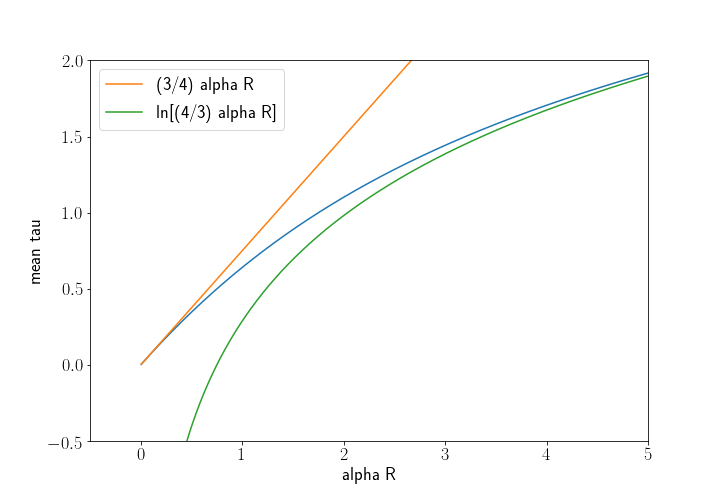
\includegraphics[width=0.9\textwidth]{tau-alphaR.png}
        \caption{ \label{fig:tau} Relationship between the mean
          optical depth and the optical depth to the center, for a
          spherical galaxy with dust and stars fully mixed. The orange
          and green lines are the optically thin and optically thick
          approximations.}
      \end{figure}

\end{document}

